\ac{LL} applications encompass a diverse range of use cases, including \ac{CG}, \ac{VR}, video conferencing, tele-robotics, industrial automation, and remote surgery. Although these applications share the common requirement of minimal end-to-end delay, each has unique characteristics and demands in terms of latency, throughput, and network protocols. 

Table \ref{tab:ll_applications} provides a summary of LL applications, highlighting their typical uplink and downlink bitrate requirements as well as the range of end-to-end latency values and compare it to video streaming which is non-interactive application.
% remove video streaming
\begin{table*}[!ht]
\setlength\tabcolsep{1pt} 
    
\begin{tabular*}{\linewidth}{@{\extracolsep{\fill}} llll}
    \toprule
       \bf LL & \bf Uplink & \bf Downlink & \bf End-to-end \\
       \bf Application & \bf Bitrate (Mbps) & \bf Bitrate (Mbps) & \bf Latency (ms) \\
    \addlinespace
    \cmidrule{1-4}
    \bf Video streaming & 0.5-3  & 3-25 & $\geq$ 300 (non interactive) \\
    \cmidrule{1-4}
    \bf Video conference & 1-3 & 1-4 & $\leq$ 300 \\
    \bf Cloud Gaming  & 2-5 & 3-40 & $\leq$ 60-100 \\
    \bf Cloud VR & 10 &  25-100 & $\leq$ 20 \\
    \bf Medical surgery & 0.5-10 & 10-100 & $\leq$ 1 \\
    \bottomrule

\end{tabular*}
\caption{Characteristics of Low-latency applications}
\label{tab:ll_applications}
\end{table*}

In this thesis, we focus on Cloud Gaming and Cloud Virtual Reality, two of the most demanding LL applications in terms of bandwidth and latency requirements. Unlike mission-critical applications such as remote medical surgery, CG and Cloud VR have established commercial implementations and deployments, providing a practical foundation for realistic experiments. These applications also represent significant business opportunities for network operators like Orange, as addressing the challenges they present is crucial for enhancing user experience and meeting the growing demand for LL services.
% specifier pourquoi cd et cloud vr avec l'interet pour orange et les challenges (justification)

\subsection{Cloud gaming}

\ac{CG} (sometimes referred to as game streaming) is a gaming paradigm where the player sends its game commands to a server located in the cloud that executes the game and produces video frames that is streamed back to the player. This gaming paradigm implies that powerful computing resources such as \ac{GPU}, are no longer required by gamers as \ac{CG} can be operated on a wide range of devices such as smartphones or thin clients.
\ac{CG} arise with cloud computing and the first commercial cloud gaming platforms were OnLive and Gaikai \cite{onlive, Gaikai}.
Recent years have seen new entrants in the \ac{CG} markets. Sony acquired Gaikai in 2014 and launched \ac{PSN} \footnote{that have now merged with PlayStation Plus} and were followed by other big industry names such as Google that launched \ac{STD} \footnote{was shutted down on January 2023} (2019), Microsoft with \ac{XC} (2020), Nvidia with \ac{GFN} (2020) or Amazon with Luna (2020) \footnote{was launched in EU on March 2023} \cite{googleStadiaService, xboxXboxCloud, nvidiaNVIDIAGeForce, amazonAmazonLuna}.


\subsubsection{CG platform architecture and network protocols}
As shown in Fig. \ref{fig:chap_1:cg_architecture}, a CG architecture consists of a thin client and a cloud game server. The gamer commands acquired through game controllers, keyboards, etc. are encapsulated in network packets and sent to the cloud server. When received by the server, they are processed by the game engine to generate the game state that will be rendered and encoded to a video. This video is streamed to the client where the video frame is decoded, rendered and displayed on the thin client.

\begin{figure*}[!ht]
    \centering
    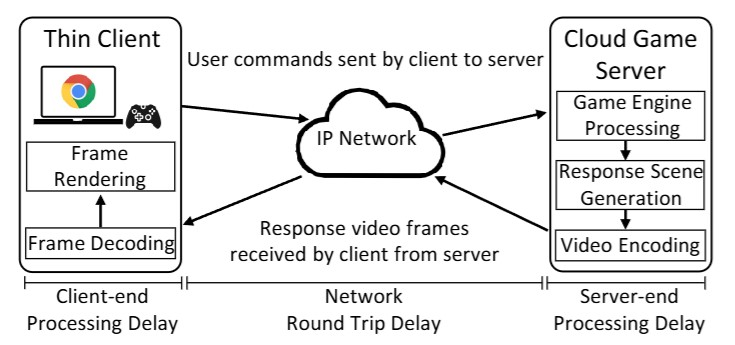
\includegraphics[width=.8\linewidth]{imgs/chapter_1/archi_cg.jpg}
    \caption{Cloud Gaming platform architecture \protect{\cite{Iqbal2021DissectingCG}}}
    \label{fig:chap_1:cg_architecture}
\end{figure*}

Commercial platforms, despite having the same broad architecture, have their specificities in terms of network protocols \cite{Iqbal2021DissectingCG, marchal2023analysis, Domenico2021ANA}. For instance, \ac{STD} and \ac{XC} rely on WebRTC: game commands are sent with \ac{DTLS} packets, video packets are encoded using H.264 and VP9 codecs and streamed using \ac{RTP} packets. \ac{GFN} uses \ac{UDP} to send user commands and also RTP for video streaming encoded using H.264 codecs. \ac{PSN} uses a custom implementation of \ac{UDP}.

Each platform specifies minimum bandwidth requirements for an optimal cloud gaming (CG) experience. However, they do not provide clear information on the maximum acceptable latency  despite its significant impact on user experience, as discussed later in this section. These recommendations are summarized in Tab. \ref{tab:cg_platforms}.
\begin{table*}[!ht]
\setlength\tabcolsep{1pt} 
    
\begin{tabular*}{\linewidth}{@{\extracolsep{\fill}} llll}
    \toprule
       \bf CG platforms & \bf Minimum Bandwidth & \bf Resolution & \bf Network protocols \\
    \addlinespace
    \cmidrule{1-4}
    \bf STD & 10/20/35Mbps & 720p/1080p/4K &  WebRTC \\ 
    \bf GFN & 15/25/45Mbps & 720p/1080p/4K & UDP \\
    \bf XC & 10Mbps & 1080p & WebRTC \\
    \bf PSN & 5/15/38Mbps & 720p/1080p/4K & UDP \\
    \bf Luna & 10/35Mbps & 1080p/4K & WebRTC \\
    \bottomrule

\end{tabular*}
\caption{Commercial CG platforms}
\label{tab:cg_platforms}
\end{table*}

\subsubsection{Factors impacting QoE in CG platforms}
Although \ac{CG} can remove the need of expensive computing hardware for gaming, streaming high-quality video gaming requires reliable and low-latency connections to avoid a bad user experience. \ac{QoE} is defined by \cite{le2013qualinet} as \textit{"the degree of delight or annoyance of the user of an application or service. It results from the fulfillment of his or her expectations with respect to the utility and/or enjoyment of the application or service in the light of the user’s personality and current state."}

According to ITU-T Rec G.1032 \cite{itut1032}, the factors of a CG that can influence the \ac{QoE} can be classified into three groups:
\begin{itemize}
    \item Human factors: These are linked to the characteristics of the user, such as gaming experience, vision and auditory capabilities, or intrinsic/extrinsic motivation.
    \item Context factors: These are related to the user’s environment, such as social context or physical surroundings (e.g., room characteristics or use in mobility versus at home).
    \item System factors: These refer to the properties that \textit{"determine the technically produced quality of an application or service"} \cite{itut1032}. This includes the game being played, the gaming setup (hardware and software), network transmission, and compression.
\end{itemize}

We focus here only on the network factors that impact the most the \ac{QoE} of cloud gaming applications.
\begin{itemize}
    \item \textbf{Delay:} In cloud gaming, delay—often referred to as button-to-pixel delay—represents the time elapsed between a user action and the corresponding visual feedback on the screen. This delay (as illustrated in Fig. \ref{fig:chap_1:cg_architecture}) can be broken down into:
    \begin{itemize}
        \item Network delay: This delay is intrinsic to network communication, as data must travel between the client and server. High delays disrupt responsiveness, rendering games less playable.
        \item Client-Side delay: Delays from this end are decreasing with advances in device performance and higher display refresh rates \cite{Kmrinen2017AMS}.
        \item Server processing delay: This delay varies by game and platform, depending on the server's capabilities and load \cite{Iqbal2021DissectingCG}.
    \end{itemize}

    The impact of delay on QoE has been been widely studied. Claypool et al. \cite{Claypool2014TheEO} demonstrated that high delays significantly degrade player performance on platforms like OnLive and GamingAnywhere, particularly for genres like racing and first-person shooters, which are more latency-sensitive than role-playing or strategy games. Peñaherrera-Pulla et al. \cite{PeaherreraPulla2021MeasuringKQ} identified latency as one of the key factors to ensure the responsiveness required for CG. Xu et al. \cite{Xu2022MeasurementOT} highlighted the impact of network congestion, showing that competing traffic (like \ac{TCP} traffics) can result in buffer bloat and thus increase delays and negatively impact QoE on platforms like \ac{STD}, \ac{GFN} and Luna.

     \item \textbf{Jitter:} Jitter is a measure of how inconsistent is the delay between packets. Jitter causes the video to be stuttered instead of being smooth. While video buffering can mitigate this in non-interactive applications like streaming, jitter poses a significant challenge in CG, where it directly impacts the \ac{QoE}.  Aumont et al. \cite{Aumont2021DissectingCG} demonstrated that jitter significantly impacts the gaming experience on CG platforms like \ac{STD} and \ac{GFN}. Oliveira et al. \cite{FlanaganEffectsOJ} confirmed these findings in their experiments on STD using four different games. They observed that high jitter magnitudes deteriorate the user experience on CG.

    \item \textbf{Bitrate:} The bitrate represents the number of bits transferred per unit of time. In CG, the bitrate (limited by the available bandwidth) determines the maximum frame rate and resolution achievable by the platforms. Some studies outlined that lowering the bitrate (with some bandwidth restrictions for example) leads to lower user experience. Suznjevic et al. \cite{suznjevic2016analysis} demonstrated in a study on GFN that reducing the bandwidth results in lower graphics quality (characterized by decreased resolution and frame rates) and thus resulting in lowers QoE scores.
    In a study analyzing the behavior of CG platforms under different network conditions, Marchal et al. \cite{marchal2023analysis} found that when the available bandwidth decreases, CG platforms adapt by reducing the bitrate. This typically results in a drop in frame rate and resolution (due to a reduction of the quantization factor that is responsible for video compression). While CG platforms do not adapt the same way to this network disturbance, all experience resolution degradation and some become unplayable when the bandwidth falls below the platform bandwidth requirements. Iqbal et al. \cite{Iqbal2021DissectingCG} observed that under constrained bandwidth conditions, CG platform cannot consistently provide 1080p/60 fps streaming.


    \item \textbf{Packet loss:} occurs when one or more packets traveling a network fail to reach their destination due to network congestion, radio frequency interferences or weak radio signals. Packet loss in CG applications significantly impacts user experience as demonstrated by Jarschel et al. \cite{jarschel2013gaming} on their experiment with an emulated CG platform. They observed that even a 1\% packet loss can reduce the \ac{MOS} score from 5 (excellent) to 2 (poor). Chen et al. \cite{chen2013quality} observed, using early CG platfors like OnLive and StreamMyGame, that packet loss affects the frame rate and the graphic quality. Thieir study revealed that former CG platforms do not implement robust packet loss concealment mechanisms. Similarly, Marchal et al. \cite{marchal2023analysis} found that \ac{PSN} does not allow to launch game sessions when packet loss exceed 5\%. In contrast, it was shown in \cite{Aumont2021DissectingCG, marchal2023analysis} that modern CG platforms like STD, GFN, XC are slightly impacted by packet loss as they used resilient error correction mechanisms including \ac{FEC} and high redundancy.
\end{itemize}


% Wang et al. \cite{Wang2012CloudMG} identified the gaming visual experience and the gaming response experience as the impairment factors affecting mobile \ac{CG}. Gaming visual experience depends on the video smoothness and the image quality which are linked to the bandwidth, packet loss and the compression process from the server while gaming response depends on the end-to-end delay. 



\subsection{Cloud VR}
\ac{VR} is a computer-generated experience where users can interact and feel immersed in a virtual environment. Traditional VR applications require high-end computers for the demanding graphics and processing for 3D immersive experiences, as most VR headsets cannot handle all the heavy computations and processing. As a result, the headsets are either tethered to the computer or wireless linked via technologies like AirLink to stream content.

Cloud \ac{VR} consists in offloading all the heavy computational tasks to cloud servers enabling real-time streaming of rendered VR content to lightweight and less expensive VR headsets. This approach reduces the need for powerful and costly computers, making VR more accessible and affordable. By removing the need on tethered setups, Cloud VR offers more mobility and flexibility enabling diverse use-cases of VR experiences. Cloud VR could also support scalability and fosters collaboration, opening opportunities for enterprises and institutions to develop innovative VR services.

According to \cite{huawei}, Cloud VR applications can be classified into two categories:
\begin{itemize}
    \item Weak-interaction VR that implies no interaction with the virtual environment. The users are passive and the contents are pre-determined. This includes 360 degree panoramic video, VR streaming or VR live broadcast.
    \item Strong-interaction VR includes VR services where user can interact in real-time with virtual environments through interactive devices for greater immersion. In these applications, the virtual environment depends on the inputs of the user unlike weak-interaction. This includes VR gaming, VR social networking (metaverses) and so on.
\end{itemize}
This thesis focuses only on strong interaction VR and Cloud VR will be used to refer to strong-interaction VR unless otherwise stated. 

\subsubsection{Factors impacting QoE in Cloud VR platforms}

As for CG, ITU-T Rec G.1035 \cite{itut1035} classified the factors that can influence the QoE in cloud VR into human, context and system factors.
The network factors impacting the Cloud VR experience are categorized based on the experience evaluation factors of Cloud VR, which according to \cite{huawei} are: \textbf{i) the sense of reality} which are determined by the quality of audio and video to allow the users to feel immersed and are directly impacted by the bandwidth; \textbf{ii) the sense of interaction} which are impacted by the latency and \textbf{iii) the sense of pleasure} that depends on the smoothness and can be impacted by the bandwidth, the latency and the packet loss.
Thus, as for CG, the most influencing network factors on QoE for Cloud VR are:
\begin{itemize}
    \item \textbf{Delay:} In VR, the delay, often referred as \textit{motion-to-photon} (MTP) delay, is the time elapsed between a user movement and the resulting change in the headset's field of view after rendering. In Cloud VR, the network latency adds to MTP delay because the VR content is streamed from the cloud. The impact of delay in Cloud VR were discussed in the literature. Song et al. \cite{song2022impact} demonstrated that increased latency results in black edge artifacts (that corresponds to black area in the viewport boundary when users turn their heads) affecting QoE. Their study highlighted the sensitivity of users to both the duration and size of these artifacts. Lee et al. \cite{lee2024adaptive} found that higher delays or lower frame rates contribute to cybersickness, further degrading the VR experience. Warsinke et al. \cite{warsinke2024vr} observed that even moderate additional delays (e.g., 40 ms) significantly affect VR session quality, with impacts varying by game genre.
    
    \item \textbf{Bandwidth:} Cloud VR applications are highly bandwidth-intensive due to higher resolutions, higher frame rates, coding technology used, extra-perspective rendering and transmission required to reduce the impact of black edge events. Bandwidth constraints can lead to reduce graphics quality and frame rates, affecting the user experience. \cite{huawei} reported that a minimum bandwidth of 80 Mbps is required for a fair-experience. Li et al. \cite{li2020performance} showed that insufficient bandwidth may causes congestion, reducing frame rates and compromising QoE. Their subjective studies confirmed that users notice and react negatively to these degradations. Lee et al. \cite{lee2024adaptive} identified a direct correlation between increased bitrate and better visual quality, using the MOS score of their QoE model.  

    \item \textbf{Packet loss:} It is recommended to use UDP for Cloud VR but since there is no retransmissions in UDP, packet loss can cause issues like visual quality degradations or black edge events. Li et al. \cite{li2020performance} confirmed with objective and subjective studies that packet loss disrupts frame rates and graphics, and affects user experience. Rossi et al. \cite{rossi2024subjective} observed in a subjective study, that packet loss rates as low as 12\% adversely affect throughput and frame rate, reducing the MOS. Warsinke et al. \cite{warsinke2024vr} highlighted that even minimal packet loss (0.3\%) significantly impacts VR gaming session quality.  



\end{itemize}

% These findings collectively emphasize that delay, bandwidth, and packet loss are critical determinants of QoE in Cloud VR. Addressing these factors is essential for enhancing the user experience and mitigating performance issues in Cloud VR applications.  

% On experiments on a cloud VR gaming platform (ALVR), Li et al. \cite{li2020performance} shown in objective studies that frame rate is impacted by insufficient bandwidth and packet loss. Latency is also impacted by these parameters as lower bandwidth lead to congestion. They also conduct subjective studies and shown that gaming experience are impacted by delay, bandwidth and packet loss.


% Song et al. \cite{song2022impact} prove the relationship between latency in cloud VR and black edge artifacts (that corresponds to black area in the viewport boundary when users turn their heads). They shown in subjective studies that the QoE are impacted by the duration and also the area of a black edge event as users easily noticed black edge events.


% Rossi et al. \cite{rossi2024subjective} showed on subjective QoE tests using a commercial Cloud VR solution that round-trip time, jitter and packet loss impact the MOS score. The Cloud VR gaming throughput was impacted by jitter and packet loss rate of 12\% while the frame rate was affected by \ac{RTT}.


% Lee et al. \cite{lee2024adaptive} shown in a user studies that the MOS score increase as the bitrate increases leading to better visual quality. They also shown that the QoE depends on the game genres that may have different requirements and that cyersickness occured with higher delays or lower frame rates. They also proposed and validated a QoE model based on network parameters like bandwidth, delay and packet loss which prove that they are impacting factors for QoE.


% Warsinke et al. \cite{warsinke2024vr} design a user study and shown that packet loss (0.3\%) and additional delay (40ms) impact the overall VR gaming session quality but the results differs depenging on the game genre.

% reinsérer dans les bullet points.

% \takeaway{Low-latency applications like CG and Cloud VR demand minimal delay and high network reliability to deliver interactive and immersive experiences. Their performance is influenced by factors such as latency, jitter, bitrate, and packet loss as highlighted by many studies in the literature.}

% \takeaway{\ac{LL} applications like cloud gaming, Cloud VR, video conferencing, and remote medical surgery share a need for minimal end-to-end delay, but their bandwidth and latency requirements differ. CG and Cloud VR, the focus of this thesis, demand high network reliability to deliver interactive and immersive experiences. These applications involve complex architectures and protocols, with network factors like delay, jitter, bitrate, and packet loss significantly impacting user experience as highlighted by many studies in the literature.}

% améliorer le lien

% \usage{This thesis focuses on CG and CloudVR as \ac{LL} applications. Data collection (Chapter \ref{chap:measurements}) was performed using commercial CG platforms and experimental versions of CloudVR systems. These datasets serve as the foundation for developing anomaly detection (Chapters \ref{chap:ml_evaluation}, \ref{chap:cats}) and root-cause diagnosis techniques (Chapter \ref{chap:diagnosis}).}


% \usage{This thesis focuses on anomaly detection and root-cause diagnosis for the performance of low-latency (LL) applications, with a specific emphasis on CG and Cloud VR. These applications were chosen due to their growing business relevance for Orange and their sensitivity to network performance issues. In Chapter \ref{chap:measurements}, we conduct data collection using commercial CG platforms and experimental Cloud VR systems under time-varying network conditions. These conditions are designed to replicate real-world scenarios prone to the network factors which can cause performance anomalies in LL applications. The resulting datasets provide the foundation for evaluating anomaly detection techniques in Chapters \ref{chap:ml_evaluation} and \ref{chap:cats}. Furthermore, they are used to evaluate our proposed solution for root-cause diagnosis of LL application performance issues, detailed in Chapter \ref{chap:diagnosis}.}